\chapter{NAO Kinematics: The Results}
\label{Results}

There are several ways to validate solutions to forward and inverse kinematics and verify that the method used works properly. The verification of forward kinematics is trivial; we just move the end effector of a kinematic chain to a point and we check if forward kinematics returns the correct position and orientation. On the other hand, verification of inverse kinematics is more difficult, because we must give a valid (accessible) target point as input, otherwise inverse kinematics cannot find a solution.

A practical problem is there is no clear way to know the exact work space for the end effectors of NAO. Therefore, we came up with another way of verifying our solution. We manually move an end effector to a random point, we read off the position and the orientation of this point from the forward kinematics, and then we assign this point as the target point for inverse kinematics. Finally, we check if inverse kinematics finds a solution and we know right away that this solution is correct, because the solution is check through forward kinematics against the given target point before returned.

We created two demonstrations to show the effectiveness and the efficiency of our kinematics in the real world. The first demonstration is a pointing-to-the-ball task, whereby a standing robot tracks a ball in the field and uses forward kinematics of the legs and inverse kinematics of the arms to point to the exact location of the ball with its extended arm(s). The second demonstration is more complicated and consists of a simple balancing method, whereby the robot calculates its current center of mass through forward kinematics and drives one of its legs to the projection of the center of mass on the floor using inverse kinematics to maintain balance.


\section{Real-Time Performance}
One of the goals of this work was to implement a software library for real-time kinematics computations on the robot. We measured the performance of our implementation for each of the functions we offer. Table~\ref{times} shows average execution times for each function in microseconds (us). Averages were taken over 6000 measurements of execution time on the robot CPU. Unfortunately, we cannot compare these times with Aldebaran's solution execution time, because we no access inside the proprietary NaoQi middleware. 

%\begin{table}[!t]
%\centering
%\caption{Execution Times}
%\vspace*{0.06cm}
%\begin{tabular}{|l|c|}
%\hline
%\textbf{Function} & \textbf{Time (us)}\\ \hline
%Forward For Head & 54.28 \\
%Forward For Left Arm & 66.72 \\
%Forward For Right Arm & 69.54 \\
%Forward For Left Leg & 80.88 \\
%Forward For Right Leg & 80.78 \\
%Inverse For Head & 70.79 \\
%Inverse For Left Arm & 170.55 \\
%Inverse For Right Arm & 200.00 \\
%Inverse For Left Leg & 185.29 \\
%Inverse For Right Leg & 184.85 \\
%Calculation of CoM & 394.55 \\
%\hline
%\end{tabular}
%\label{times}
%\end{table}

\begin{table}[!t]
\caption{On-board execution times of the NAO kinematics library}
\label{times}
\begin{center}
\begin{tabularx}{9.3cm}{lc}
\toprule%
\textbf{Kinematics Function} & \textbf{Time (us)}\\
\midrule [\heavyrulewidth]%
Forward Kinematics for Head & 54.28 \\
Forward Kinematics for Left Arm & 66.72 \\
Forward Kinematics for Right Arm & 69.54 \\
Forward Kinematics for Left Leg & 80.88 \\
Forward Kinematics for Right Leg & 80.78 \\
Inverse Kinematics for Head & 70.79 \\
Inverse Kinematics for Left Arm & 170.55 \\
Inverse Kinematics for Right Arm & 200.00 \\
Inverse Kinematics for Left Leg & 185.29 \\
Inverse Kinematics for Right Leg & 184.85 \\
Calculation of the Center of Mass & 394.55 \\
\bottomrule%
\end{tabularx}
\end{center}
\end{table}


\section{Locus of Problematic Inverse Kinematics}
\label{undefined}
As mentioned in Section~\ref{invleftleg}, there are a few target points for the legs which lead to an infinity of solutions for the AnkleRoll joints, while the KneePitch and AnklePitch joints take specific values. Even though this is not a problem, to verify that in practice the robot never reaches any of these configurations, we let the robot perform the entire range of motions available to it during operation in a RoboCup field (walk, kicks, stand-up, etc.). We recorded all configurations encountered in the KneePitch and AnklePitch subspace of both legs and we plotted these configurations alongside the locus of the problematic configurations. The results are shown in Figure~\ref{fig:undefined}. It is clear that no motion brought the robot to these configurations. In practice, it is rather unlike that anyone will consistently give target points that drive the joints in that area. This is true, because, when executing a trajectory, inverse kinematics are called on a sequence of target points (at a frequency of 50 to 100 Hz), so even if one of them falls right into the problematic fraction of the three-dimensional space, it is highly unlike that the next one will do the same. At such a high frequency, the problematic solution will go unnoticed and the motion will proceed smoothly.

\begin{figure}[h]
	\begin{center}
		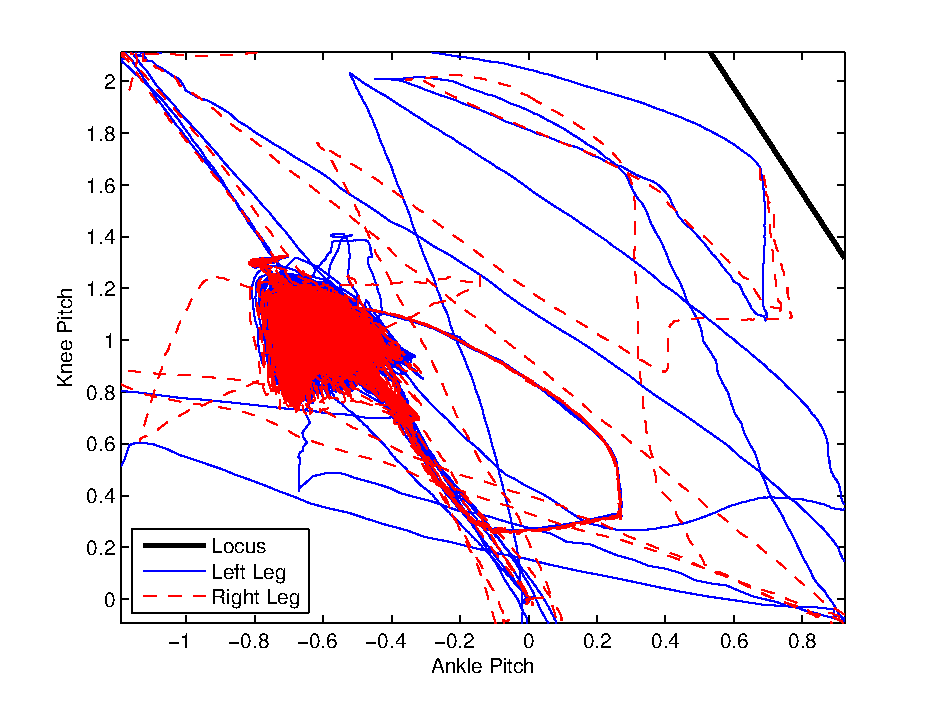
\includegraphics[width=\textwidth]{Figures/undefined.pdf}
 		\caption{Trajectories of motion in a subspace of the leg joints}
 		\label{fig:undefined}
	\end{center}
\end{figure}

\newpage


\section{Demonstration I: Pointing to the Ball}

In the first demonstration, our goal is to make the NAO point to the ball with its stretched arms. Apart from the kinematics, to realize this task we employed the KVision module~\cite{orfanoudakis2011} for ball recognition of the Kouretes team, along with the module that updates the local world state belief of the robot. Initially, NAO searches for the ball by scanning the field with its head. When it finds the ball, it points directly to the ball with the left, the right, or both arms, depending on where the ball is located (left, right, or front). Thanks to the filtering of the world state module, if NAO loses momentarily the ball from its visual field, it can continue pointing to the location indicated by the ball model. 


\begin{figure}[!t]
\centerline{
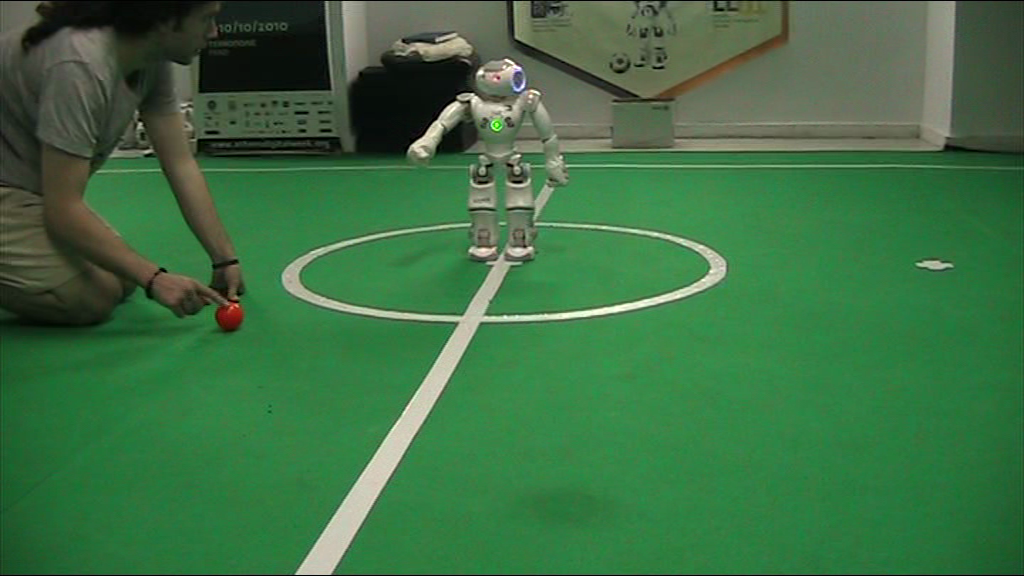
\includegraphics[width=0.32\textwidth]{Figures/Demo1/1.png}
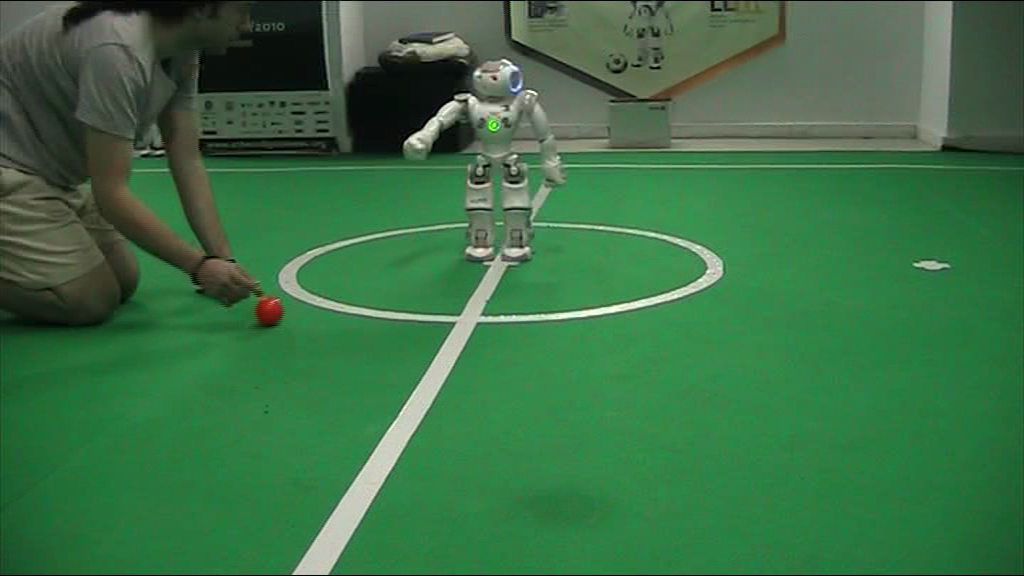
\includegraphics[width=0.32\textwidth]{Figures/Demo1/2.png}
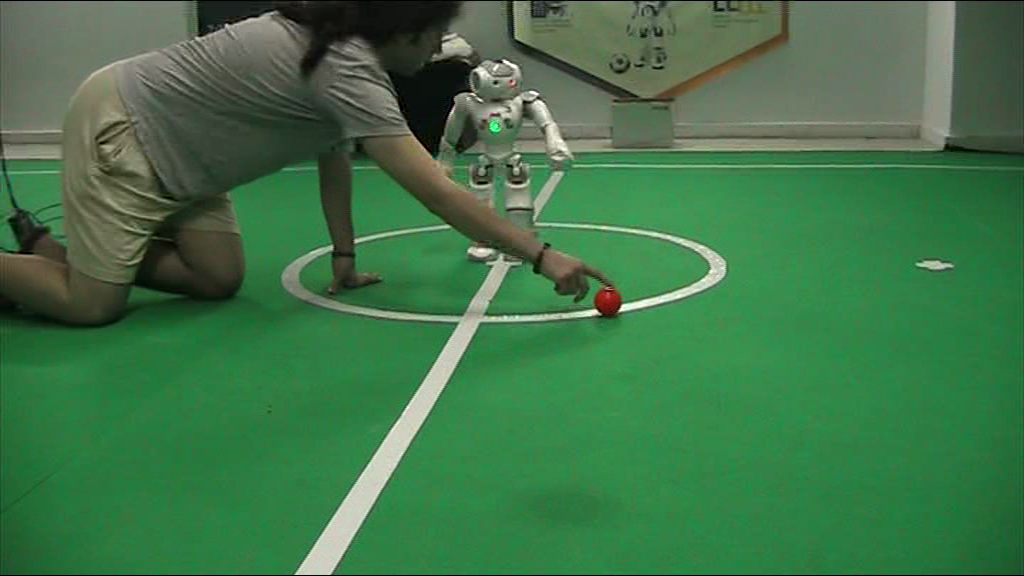
\includegraphics[width=0.32\textwidth]{Figures/Demo1/3.png}
}
\vspace*{0.06cm}
\centerline{
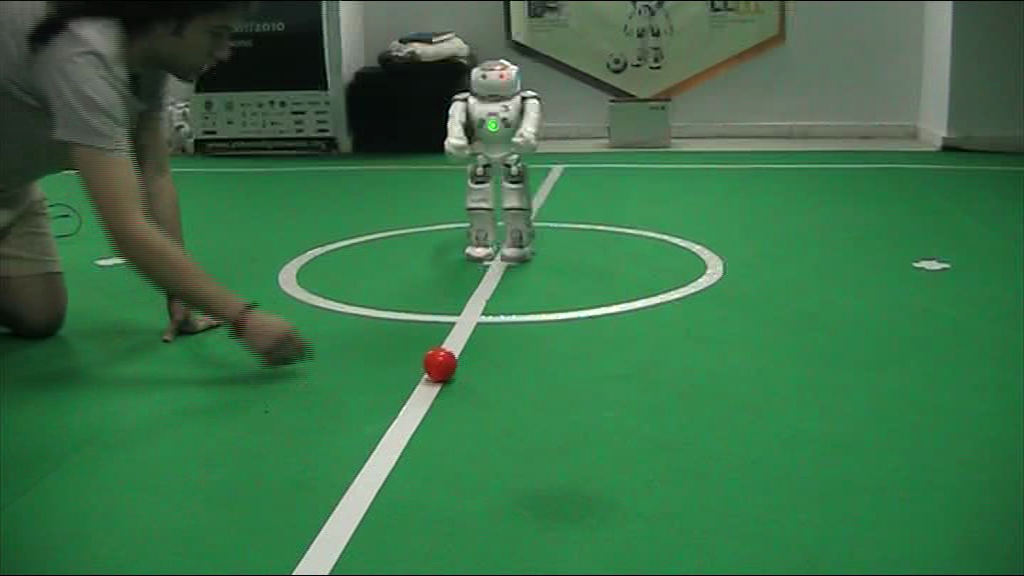
\includegraphics[width=0.32\textwidth]{Figures/Demo1/4.png}
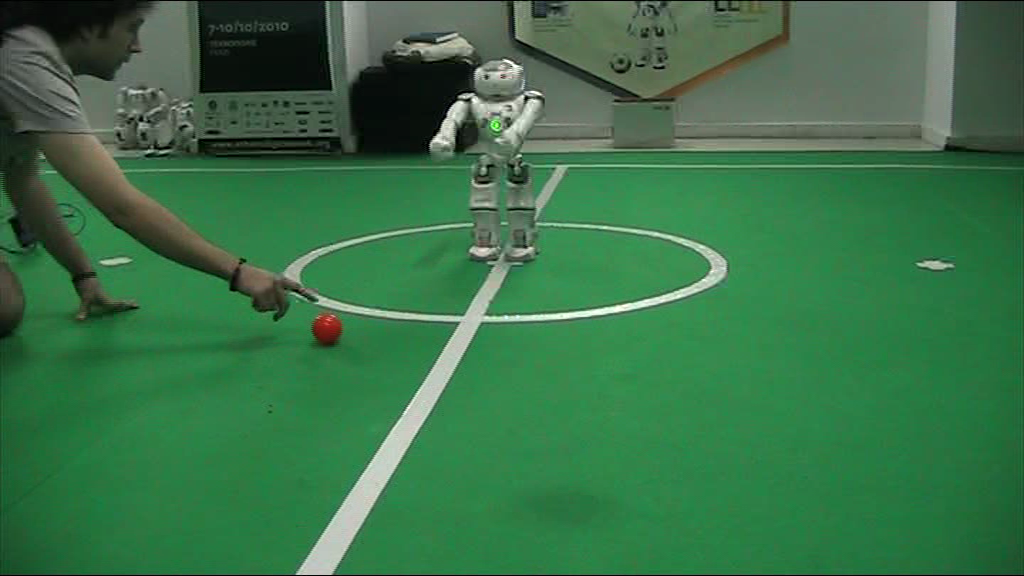
\includegraphics[width=0.32\textwidth]{Figures/Demo1/5.png}
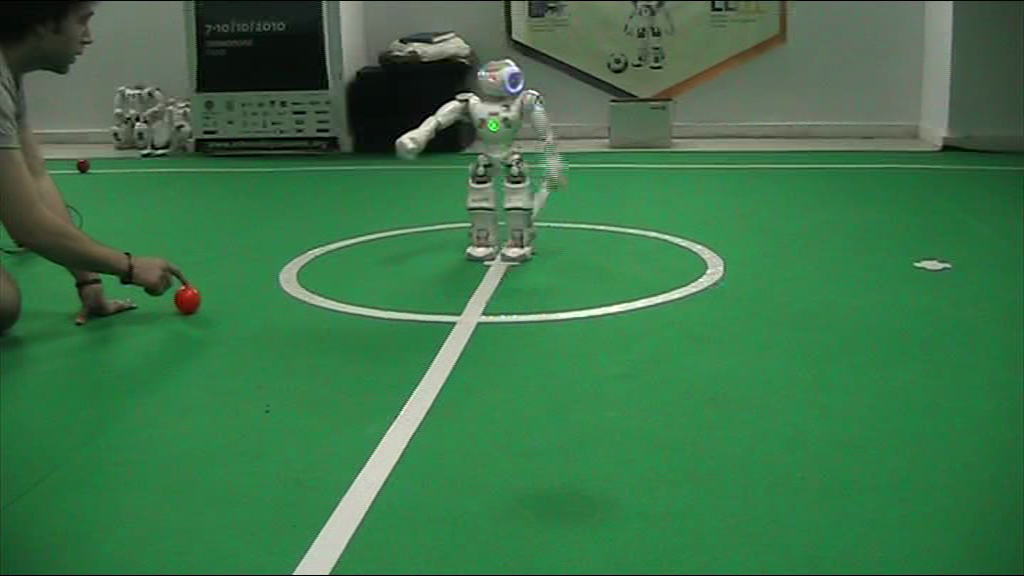
\includegraphics[width=0.32\textwidth]{Figures/Demo1/6.png}
}
%\vspace{-0.1cm}
\caption{Pointing to the ball with the NAO using forward and inverse kinematics}
\label{demo1}
%\vspace*{0.5cm}
\end{figure}

The ball observation can be described as a two-dimensional point without orientation. The location of the ball is given in polar coordinates, that is distance and bearing relatively to the projection of the robot torso on the floor. We must now transform this point from the two dimensions to the three dimensions and give it an orientation. To do so, we transform the polar coordinates to Cartesian coordinates $(p_x,p_y)$ and we add the height of the torso as the third coordinate $p_z$ to form the ball position $(p_x,p_y,p_z)$ in the three-dimensional space.  We also know that $a_x$ equals to zero, because we are only rotating about the $y$-axis (up/down) and the $z$-axis (right/left). To find the two other orientations, we focus on the straight line that connects the position of the ball and the position of the ShoulderPitch joint relatively to the torso frame. The orientation $a_y$ is the angle between this line and the $y$-axis and the orientation $a_z$ is the angle between this line and the $z$-axis. Additionally, the position of the target point lies along this line at a distance $d$ from the ShoulderPitch joint, where $d$ is the total length of the stretched arm. We need to set the target point at that distance to make it a valid target point for inverse kinematics. We run this procedure twice, once for each arm (the difference is the position of the corresponding ShoulderPitch joints), and finally obtain the solution(s) from inverse kinematics for the left and right arms for the corresponding target points. If both solutions are returned, the robot raises both arms pointing to the ball. If only one solution is returned, the robot raises only one arm; the other arm cannot point to the ball, as it is not possible to reach the correct target point due to physical constraints. Figure~\ref{demo1} shows snapshots from this demonstration.

This demonstration was presented by team Kouretes at the SPL Open Challenge Competition at RoboCup 2012 in Mexico City, Mexico. Figure~\ref{fig:open} shows a picture taken during the open challenge presentation. 

\begin{figure}[!t]
\centerline{
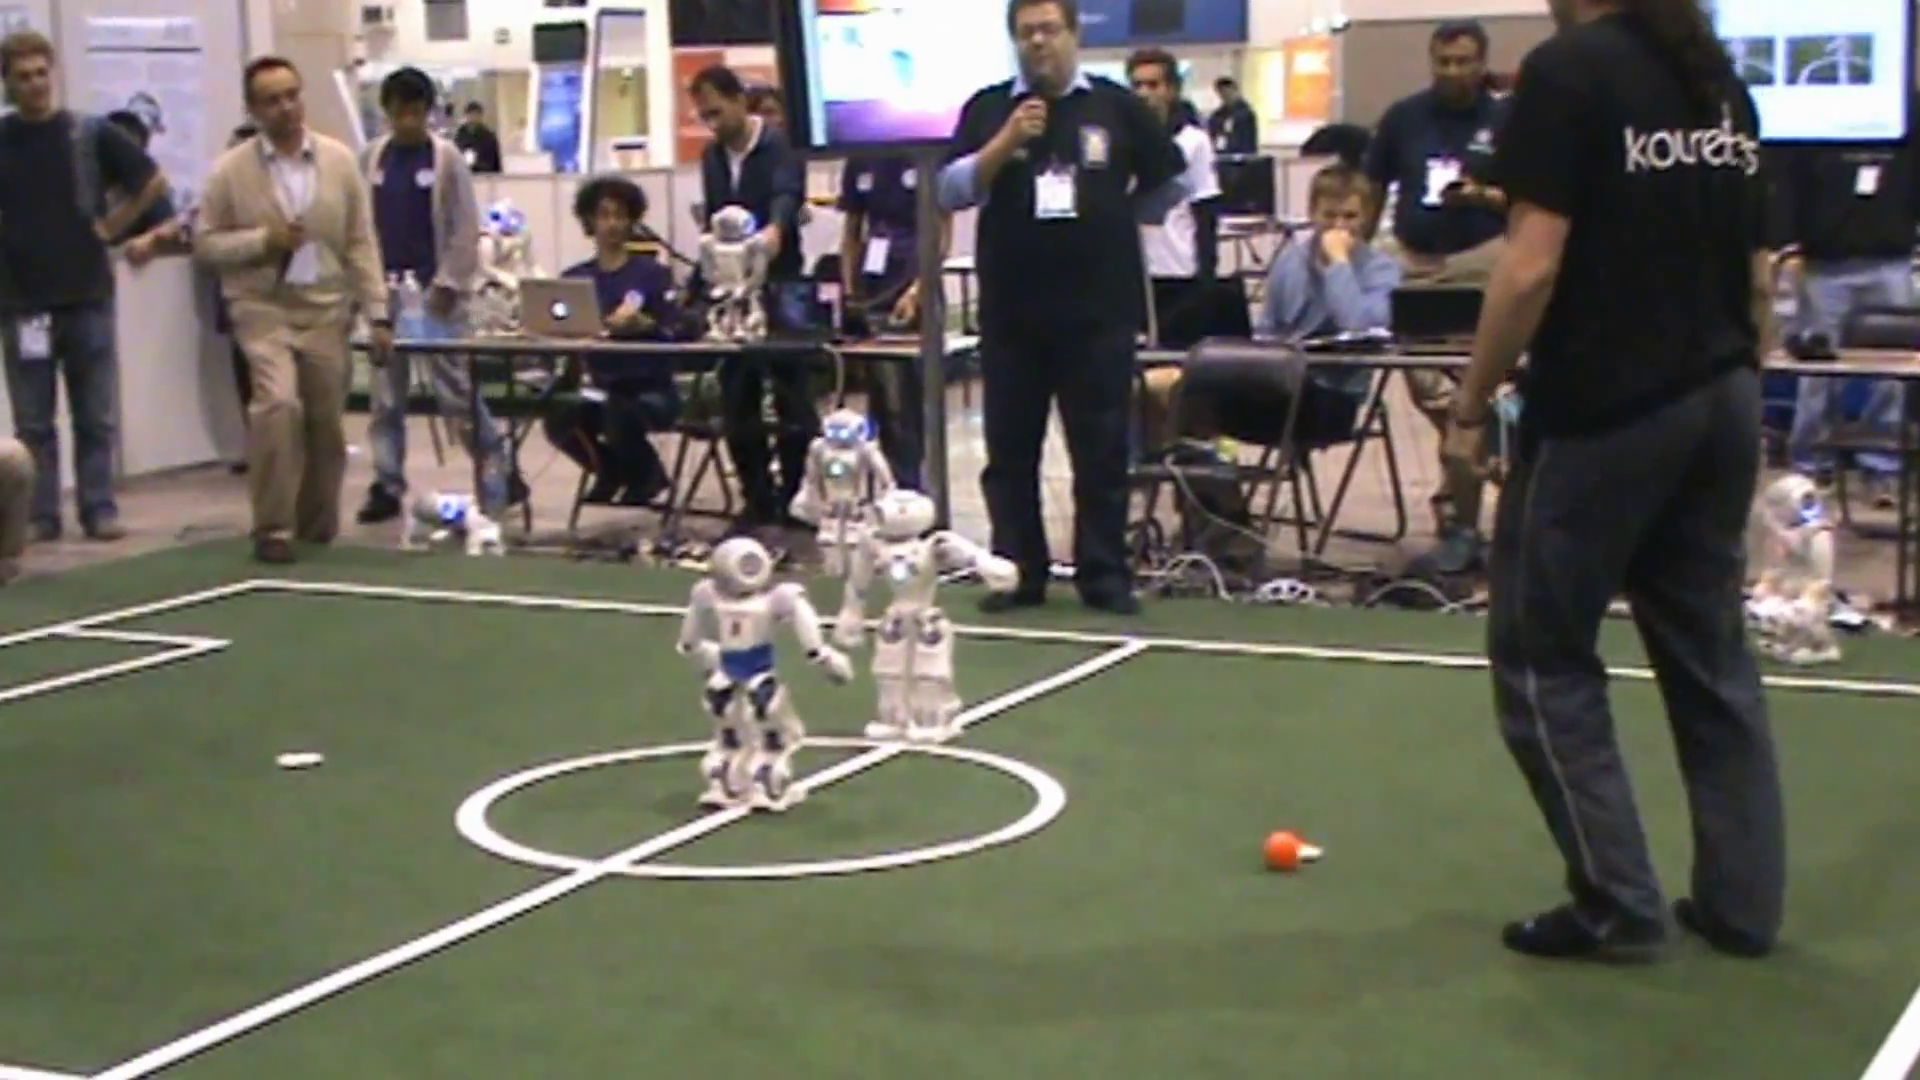
\includegraphics[width=.8\textwidth]{Figures/openchallenge2012.png}
}
\caption{Pointing to the ball at SPL Open Challenge Competition of RoboCup 2012}
\label{fig:open}
\end{figure}



\section{Demonstration II: Basic CoM Balancing}

In the second demonstration, we seek to implement a very basic balancing method. In particular, we want to make NAO move one of its feet to the point of the projection of the CoM on the floor. First, we calculate the position of the CoM using forward kinematics, which gives the CoM position relatively to the torso frame. The problem is that the $x$-$y$ plane of the torso frame is rarely parallel to the floor. Thus, we read off the inertial unit of the robot the current rotation (angleX and angleY) of the torso plane. Now, we can calculate the position of the CoM relatively to the rotated torso:
\[
	T_{\text{rotated}} = R_y(\text{angleY})R_x(\text{angleX})A_{\text{CoM}}
\]
Then, we assign a custom value to $p_z$ in $T_{(4,3)}$, which represents the desired torso height from the floor, so, and that yields $T_{\text{rotated}'}$. Now we must rotate back to the torso frame:
\[
	T_{\text{final}} = \big(R_y(\text{angleY})R_x(\text{angleX})\big)^{-1}T_{\text{rotated}'}
\]
Finally, we extract $p_x$, $p_y$, and $p_z$ from $T_{\text{final}}$ and we set $(p_x,p_y,p_z)$ as the target position for inverse kinematics. The target orientation is set to $(a_x,a_y,a_z) = (-\text{angleX}, -\text{angleY}, 0)$, because we do not care about the rotation around the $z$-axis. 

Figure~\ref{demo2} shows snapshots from this demonstration. Note that the foot is always parallel to the floor. It happens some times, that some robots have displaced inertial unit (accelerometers and gyro-meters). On these robots the foot is not parallel to the floor, but this represents a hardware problem, not a kinematics problem.

\begin{figure}[!t]
\centerline{
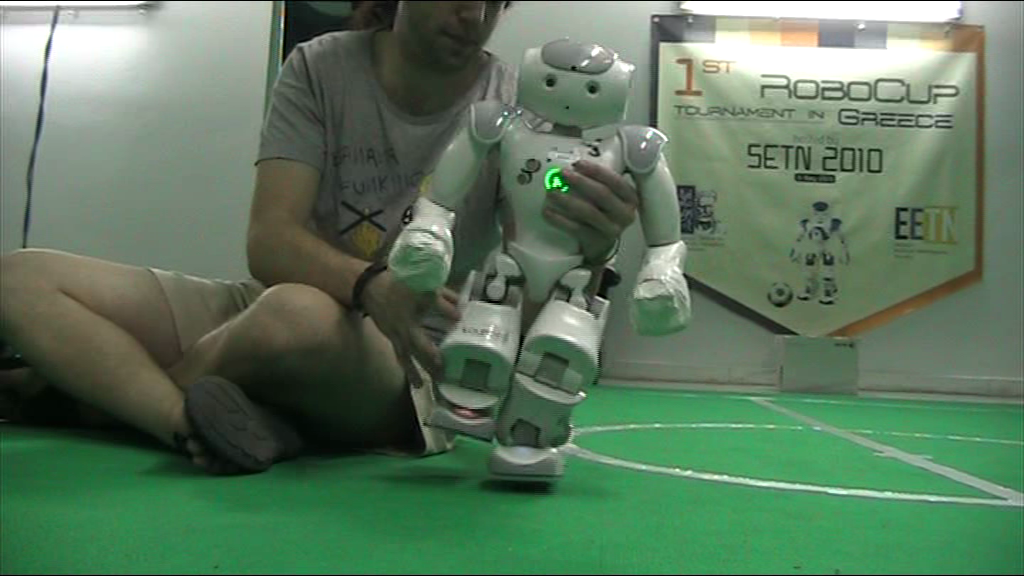
\includegraphics[width=0.32\textwidth]{Figures/Demo2/1.png}
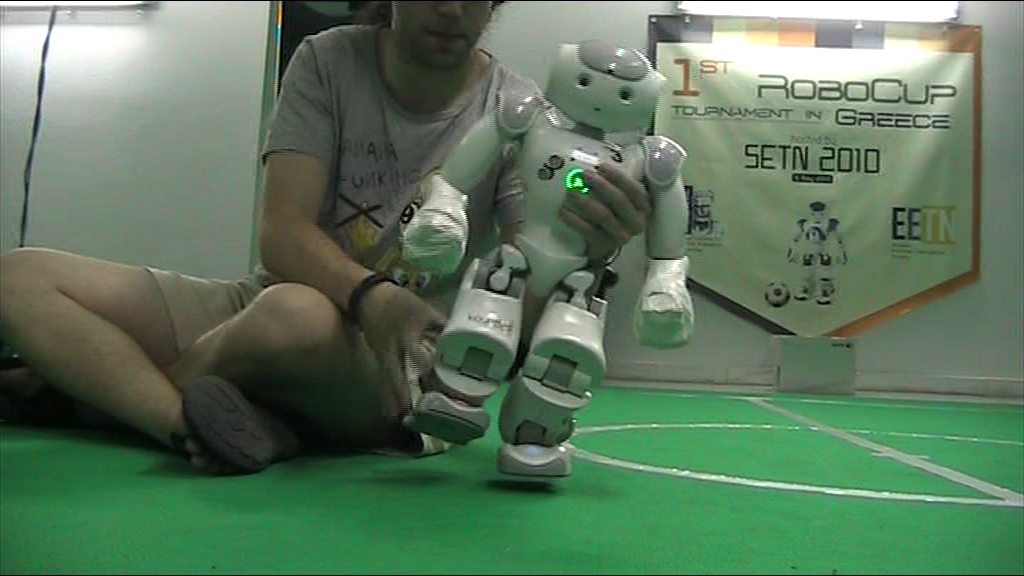
\includegraphics[width=0.32\textwidth]{Figures/Demo2/2.png}
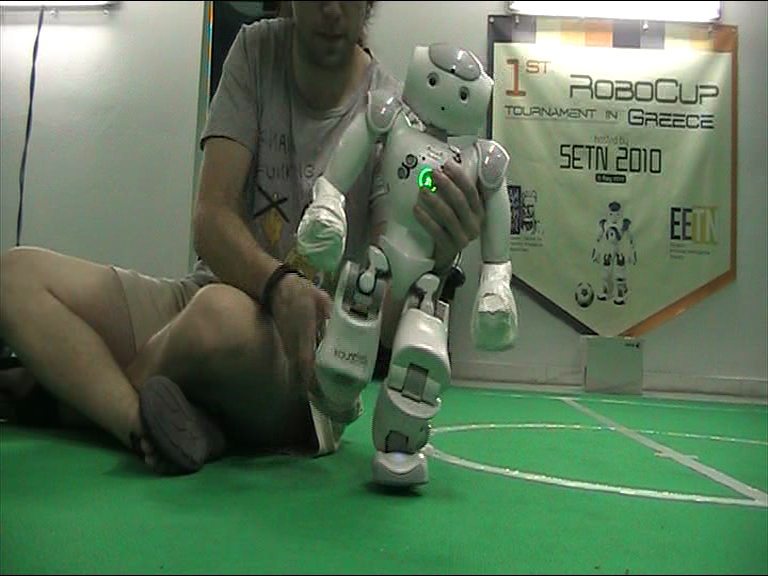
\includegraphics[width=0.32\textwidth]{Figures/Demo2/3.png}
}
\vspace*{0.06cm}
\centerline{
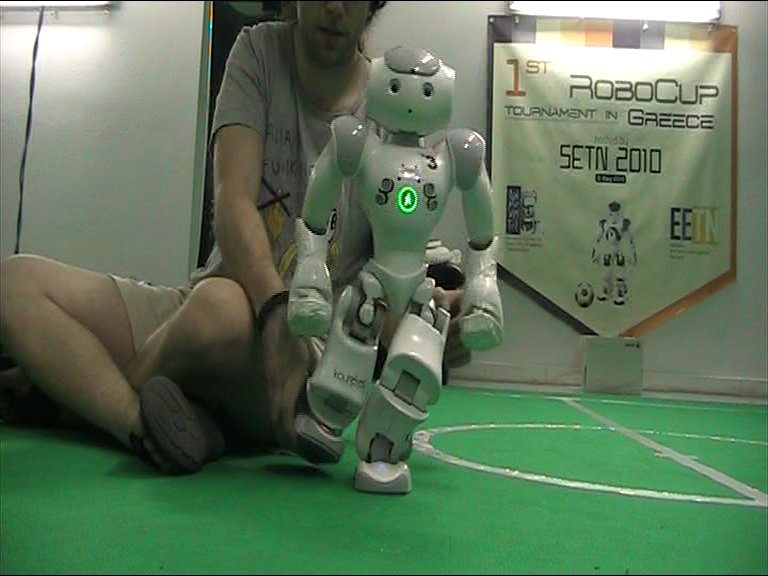
\includegraphics[width=0.32\textwidth]{Figures/Demo2/4.png}
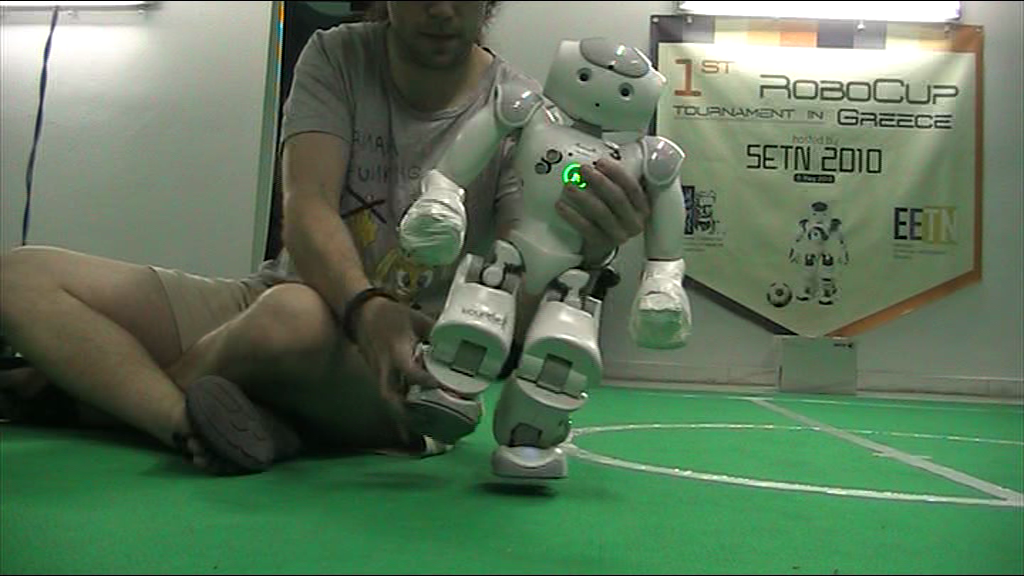
\includegraphics[width=0.32\textwidth]{Figures/Demo2/5.png}
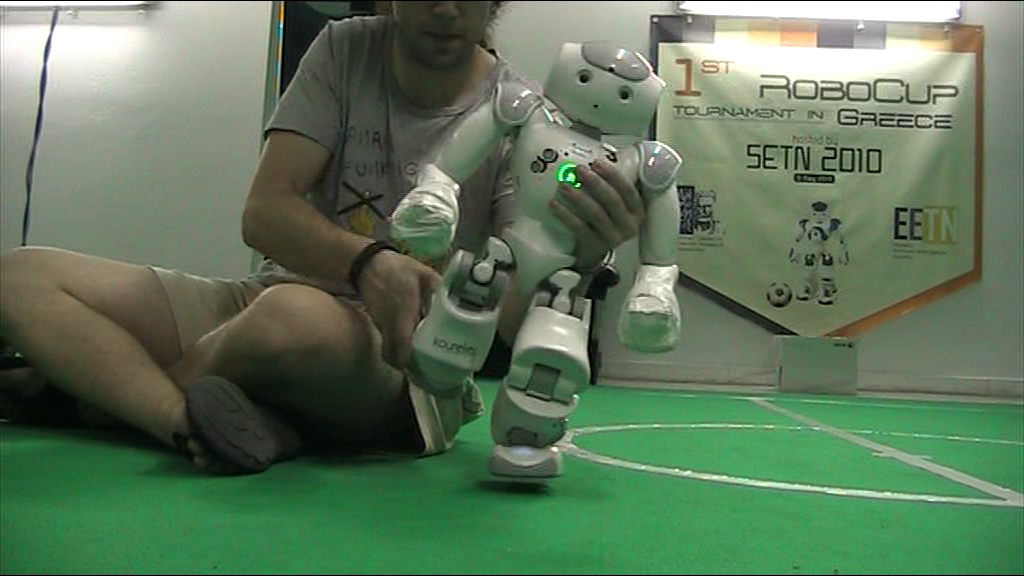
\includegraphics[width=0.32\textwidth]{Figures/Demo2/6.png}
}
%\vspace{-0.1cm}
\caption{Basic balancing for the NAO using the projection of the center of mass}
\label{demo2}
%\vspace*{0.5cm}
\end{figure}
